\documentclass[11pt]{article}            % Report class in 11 points
\parindent0pt  \parskip10pt             % make block paragraphs
\usepackage{graphicx}
\usepackage{listings}
\usepackage{tkz-graph}
\graphicspath{ {images/} }
\usepackage{graphicx} %  graphics header file
\begin{document}
\begin{titlepage}
    \centering
  \vfill
    
\includegraphics[width=8cm]{uni_logo.png} \\ 
	\vskip2cm
    {\bfseries\Large
	Data Structures and algorythm  \\ (CS09203)\\
	
	\vskip2cm
	Lab Report 
	 
	\vskip2cm
	}    

\begin{center}
\begin{tabular}{ l l  } 

Name: & MuhammadTalhaKhalid \\ 
Registration \#: &CSU-S16-135\\ 
Lab Report \#: & 9 \\ 
 Dated:& 13-04-2018\\ 
Submitted To:& Mr. Usman Ahmed\\ 

 %\hline
\end{tabular}
\end{center}
    \vfill
    The University of Lahore, Islamabad Campus\\
Department of Computer Science \& Information Technology
\end{titlepage}


    
    {\bfseries\Large
\centering
	Experiment \# 9\\

Depthh First Search in graph\\
	
	}    
 \vskip1cm
 \textbf {Objective}\\  To understand How Impliment  Depth  First Search in graph.
 
 \textbf {Software Tool} \\
1.Windows 10 \\
2. Miktex\\
3. Dev C++\\

\section{Theory }              
In this experiment we learn about Depth first search in an vector class whichis more like array but it has n fix size and  \\
It has no memory leaks because it will automaticly go to next certix if your Given dta is not there and will not search for it forever\\ \\

\section{Task}  
\subsection{Procedure: Task 1 }     
\begin{figure*}
\centering
  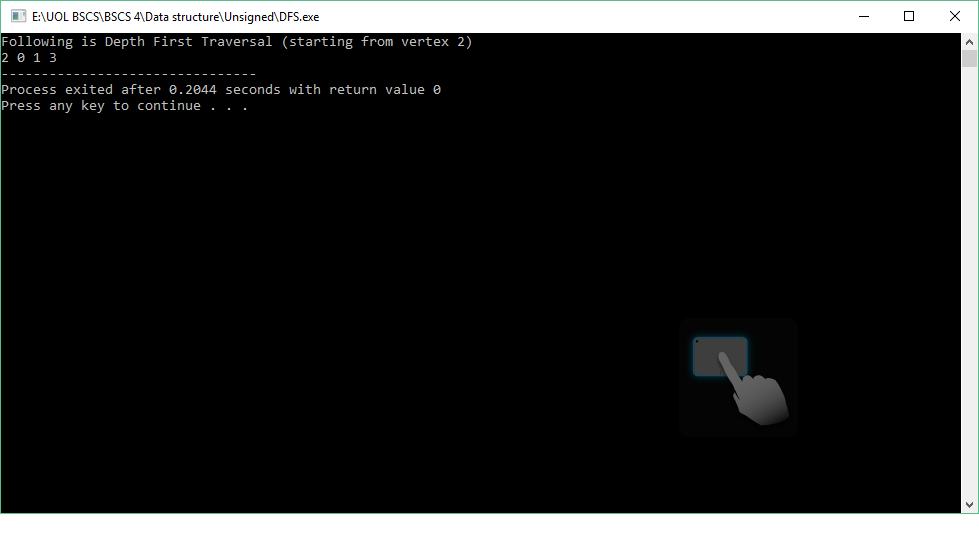
\includegraphics[width=12cm,height=6cm,keepaspectratio]{1.png}
\caption{Enter data into different location of  vertices }
\label{Figure:1}    
\end{figure*}
We have Created a class name Graph we add Vertices 'V'  and edges v and w we have created an Adjesent template pointer which actully check the direction of vector\\ 
in Depth first serch vertice 2  is  a starting point the location where we want to enter our value and the data we want to put\\
in my case i enter 1 and 2 at locationn 0,  2 at location 1,  0 and 3 at location 2 and 3 at location 3 \\
    \SetVertexSimple[MinSize=0pt] 
\subsection{Procedure: Task 2 }     
\begin{lstlisting}[language=C++]
#include<stdio.h>
#include<iostream>
#include<dos.h>
#include<unistd.h>
#include<string>
#include<stdlib.h>
#include<menu.h>
#include <list>
using namespace std;
class Graph {
private:
int V;
list <int >*adj;
void DFSUtil(int v, bool visited[]); 
public:
 Graph(int k); 
void addEdge(int v, int w);
void DFS(int v); 
};
Graph::Graph(int k) {
  this->V = k; 
 adj = new list<int>[V]; 	
	
}

 
void Graph::addEdge(int v, int w) 
{ 
    adj[v].push_back(w); 
} 

void Graph::DFSUtil(int v, bool visited[]) 
{ 
    visited[v] = true; 
    cout << v << " "; 
    list<int>::iterator i; 
    for (i = adj[v].begin(); i != adj[v].end(); ++i) 
        if (!visited[*i]) 
            DFSUtil(*i, visited); 
} 
void Graph::DFS(int v) 
{ 
    bool *visited = new bool[V]; 
    for (int i = 0; i < V; i++) 
        visited[i] = false; 
    DFSUtil(v, visited); 
} 
int main()
{
  Graph g(4); 
    g.addEdge(0, 1); 
    g.addEdge(0, 2); 
    g.addEdge(1, 2); 
    g.addEdge(2, 0); 
    g.addEdge(2, 3); 
    g.addEdge(3, 3); 
    g.DFS(2);
return 0;
}
\end{lstlisting}
\section{Graph} 
  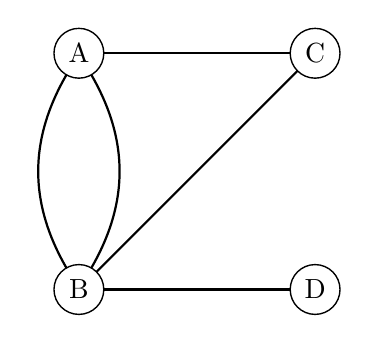
\begin{tikzpicture}
        \Vertex[x=4,y=4]{A}  
        \Vertex[x=4,y=1]{B} 
        \Vertex[x=7,y=4]{C}
	\Vertex[x=7,y=1]{D}
        \Edge[style={bend left}](B)(A)
        \Edge[style={bend right}](B)(A)
        \Edges(A,C)
        \Edges(C,B)
	\Edges(D,B)
         \Edges(D,D)
    \end{tikzpicture}

\section{Conclusion}  So in this Experiment we learn how to store our data into different location and search for it using concept of DFS Deapth fiirst search
it is quiet usefull in data structures and to create a maze teleportation in games and menipulate our large ammount of data
it is also use in Machine learning and Artificial intelligence. \\ \\ 
\end{document}                          % The required last line
